\subsection{Research-Creation Orientation}

As already mentioned, this research adopts a "research-creation" orientation. An approach that fundamentally challenges conventional divisions between artistic practice and scholarly inquiry within academic contexts  \parencite{Loveless_2019}. This approach also positions artistic practice a legitimate form of knowledge production and dissemination in its own right. This orientation operates through what Loveless terms polydisciplinamory or navigating multiple simultaneous commitments across disciplines, methods, and forms rather than maintaining allegiance to singular disciplinary frameworks \parencite[62-76]{Loveless_2019}. Another crucial bit to understand here, is that research-creation attempts to not simply add artistic components to conventional, more scientifically-oriented scholarship. Instead, it asks that practices emerge from situated, embodied engagements where form and content co-constitute one another. %Ultimately, it hopes to reshape practices that work micropolitically within university knowledge-making spaces and infrastructures \parencite[102]{Loveless_2019}.

The chosen research-creation orientation necessitates developing Speculocultural Technopoiesis (ST) as both a methodological "systematic framework" and as a form of embodied practice itself. ST aims to make apparent research-creation principles through structured protocols enabling speculocultural imagination and embodied technological practices to mutually and cyclically inform one another. As demonstrated with Figure \ref{fig:concept-architecture} the framework establishes reciprocal relationships between two primary components: the \emph{Speculocultural} dimension and the \emph{Technopoietic} dimension. These components operate in continuous dialogue. This integration manifests through ST's four-phase iterative cycle (see Figure \ref{fig:cyclical-process}). Each phase suggests specific procedures, this is to ensure that the research emerges organically and  responsively from the work itself; as opposed to emerging from predetermined frameworks. The ultimate goal it to maintain rigorous accountability to both the cultural epistemologies and material conditions animating the investigation, all the while allowing practices to follow polymorphous desires and unexpected directions (the basis of experimental practice).

\subsection{Situated/Embodied Knowledge and Reflexivity}

This research grounds itself in situated and embodied knowledge production. This is most directly needed to understand methodology (and more specifically the methods appropriated or invented for this study) as more than a disembodied set of procedures. But, instead, to understand methodology as an emerging from the specifics of positionality and lived experience required for this form of research. As a Black scholar-practitioner working with digital signal technologies, my knowledge emerges from what Manning and Massumi describe as "thinking-feeling;" that is, the inseparability of conceptual work from bodily, sensorial engagement \parencites[41-42]{Manning_Massumi_2014}. This approach is a refusal of the Cartesian split. It is a recognition that research insights arise through embodied practices of making, listening, and moving. Reflexivity also operates here in this space as well, and it is a very important operation. It provides an undulating self-reflection, similar to what Sengers et al. term "reflection-in-action," an ongoing critical awareness folded into every moment of technical and creative work \parencites[52]{Sengers_2004}. Drawing on critical theory's recognition that "our everyday values, practices, perspectives, and sense of agency and self are strongly shaped by forces and agendas of which we are normally unaware," reflective design provides means to gain awareness of such forces as a first step toward possible change \parencites[50]{Sengers_2004}. For me, this means a continuous interrogation of how my own cultural positioning, technical assumptions, and aesthetic preferences may shape what I notice, how I chose to modify tools, and what I consider a successful outcome. The autoethnographic-ness of ST requires conditions for this reflexivity. This will be achieved through systematic documentation of decision-making processes, affective responses, and "sit-ins" with moments of friction between cultural knowledge and technical constraint. This is in an effort to make visible the "unconscious values embedded in computing and the practices that it supports" \parencites[49]{Sengers_2004}.

 ST's four domains: \emph{Fugitive Speculation} (FS), \emph{Material Memory} (MM), \emph{Sensory Worlding} (SW), and \emph{Intimate Witnessing} (IW) (see Figure \ref{fig:main-domains}), aims to operationalize situated and embodied knowledge as part of the methodological practice. The solo, the reflective practice, and in collaboration, the small-cohort structure, creates conditions for what Manning and Massumi term "emergent attunement." This is described as a collective calibration of whether modifications successfully embody intended cultural logics \parencites[117-120]{Manning_Massumi_2014}. Together, with the domains, we aim to ensure that situated knowledge remains operational throughout the research cycle, preventing any potential collapse back into disembodied proceduralism. This also helps to maintain yet another aspect of the  methodological research rigor, by culturally grounding the criteria for which evaluation and iteration emerge. 

\subsection{Cyclical Process - The Four ST Cycle Phases}

\begin{figure}[H]
	\centering
	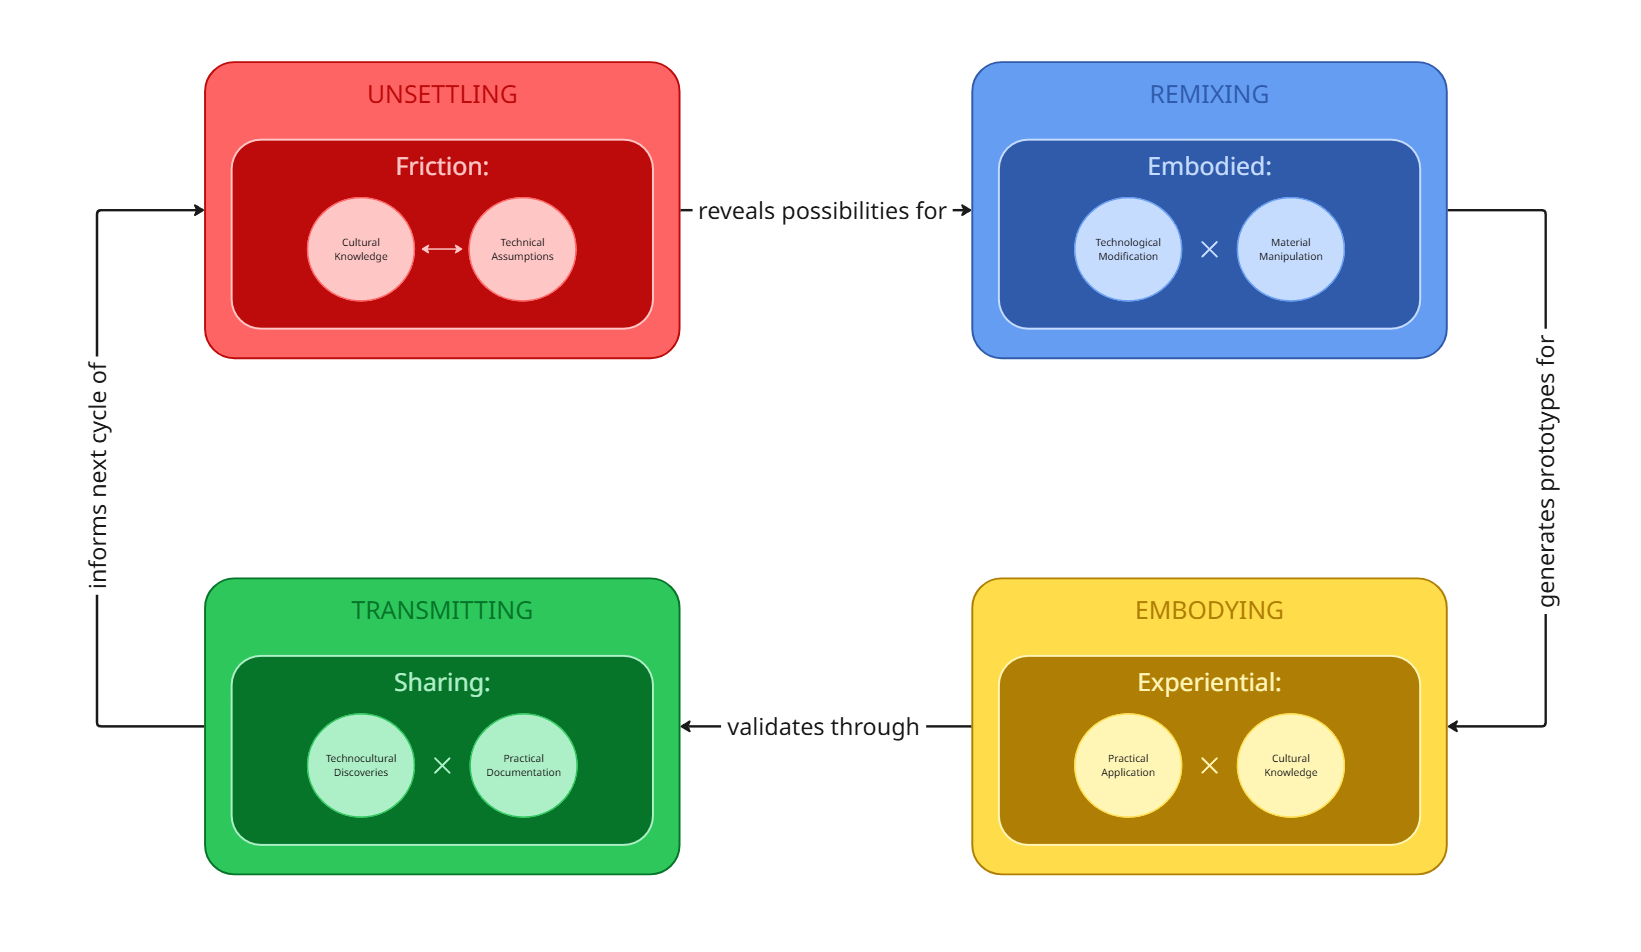
\includegraphics[width=.85\textwidth]{assets/figures/st_process.png}
	\caption{The four main movements of the cyclical process of ST in practice}
	\label{fig:cyclical-process}
\end{figure}

\subsubsection{Unsettling}
\noindent Unsettling (U) is a affect that arises when the embodied lived experience encounters, often in unsatisfactory ways, the hidden assumptions of technological toolsets. Unsettling is about encountering and categorizing the \textit{frictions} between cultural embodied knowledge and technological assumptions.
\begin{comment}
\begin{itemize}[noitemsep]
	\item Systematic identification and documentation of cultural assumptions embedded in digital audio tools
	\item Archaeology revealing biases in existing processing paradigms and interface design
	\item Critical analysis procedures for questioning technological defaults
\end{itemize}
\end{comment}
 
\subsubsection{Remixing}
\noindent Remixing (R) is a form of \textit{embodied modification}, and \textit{material manipulation} that results in knowledge creation. It encompasses the development of the "alternative" and the discovery of the "unauthorized". This form of knowledge arises not by traditional academic paradigmatic means of making technologies "more efficient" or being grounded in capitalist desires of product. Rather, these arise from making technologies "work differently" through specific epistemologies and the cultural need(s).
\begin{comment} 
\begin{itemize}[noitemsep]
	\item Systematic approaches to sampling, layering, and recombining existing computational elements
	\item Collaborative modification processes enabling community adaptation of tools
	\item Generative procedures creating new forms through computational combination guided by cultural knowledge
\end{itemize}
\end{comment}

\subsubsection{Embodying}
\noindent Embodying (E) is concerned with the functionality of tools more so as a form of cultural authenticity over technicality. It serves as a means of testing and validation through practice and creation with modified toolsets. Embodying means asks questions: "Does this modification feel genuine to the cultural knowledge that guided its creation?" or "Does it enable forms of expression that honor the epistemological foundations it draws from?" The form of knowledge validation sought through embodied engagement, not theoretical analysis.
\begin{comment}      
\begin{itemize}[noitemsep]
	\item Algorithms derived from embodied cultural knowledge and physical sonic practices
	\item Procedural systems where bodies become primary sites of technological knowledge
	\item Computational logic based on movement, gesture, and sensory sonic experience
\end{itemize}
\end{comment}

\subsubsection{Transmitting}
\noindent Transmission (T) occurs when successful cultural-technical discoveries become a part of, or solo, methodologies individuals of the a kin communities' can adapt with relative ease and understanding. The form of knowledge sharing that occurs not only preserves the techniques, but the cultural reasoning behind them; that knowledge transfer maintains epistemological integrity while enabling broader adaptation or further experimentation/iteration.
\begin{comment}      
\begin{itemize}[noitemsep]
	\item Distributed procedural processing enabling knowledge sharing
	\item Systems designed for collaborative modification and collective development
	\item Procedural approaches facilitating connection between individual practice and collaborative creation
\end{itemize}
\end{comment}

\subsection{Guiding Dimensions - The Four ST Domains}

\begin{figure}[H]
	\centering
	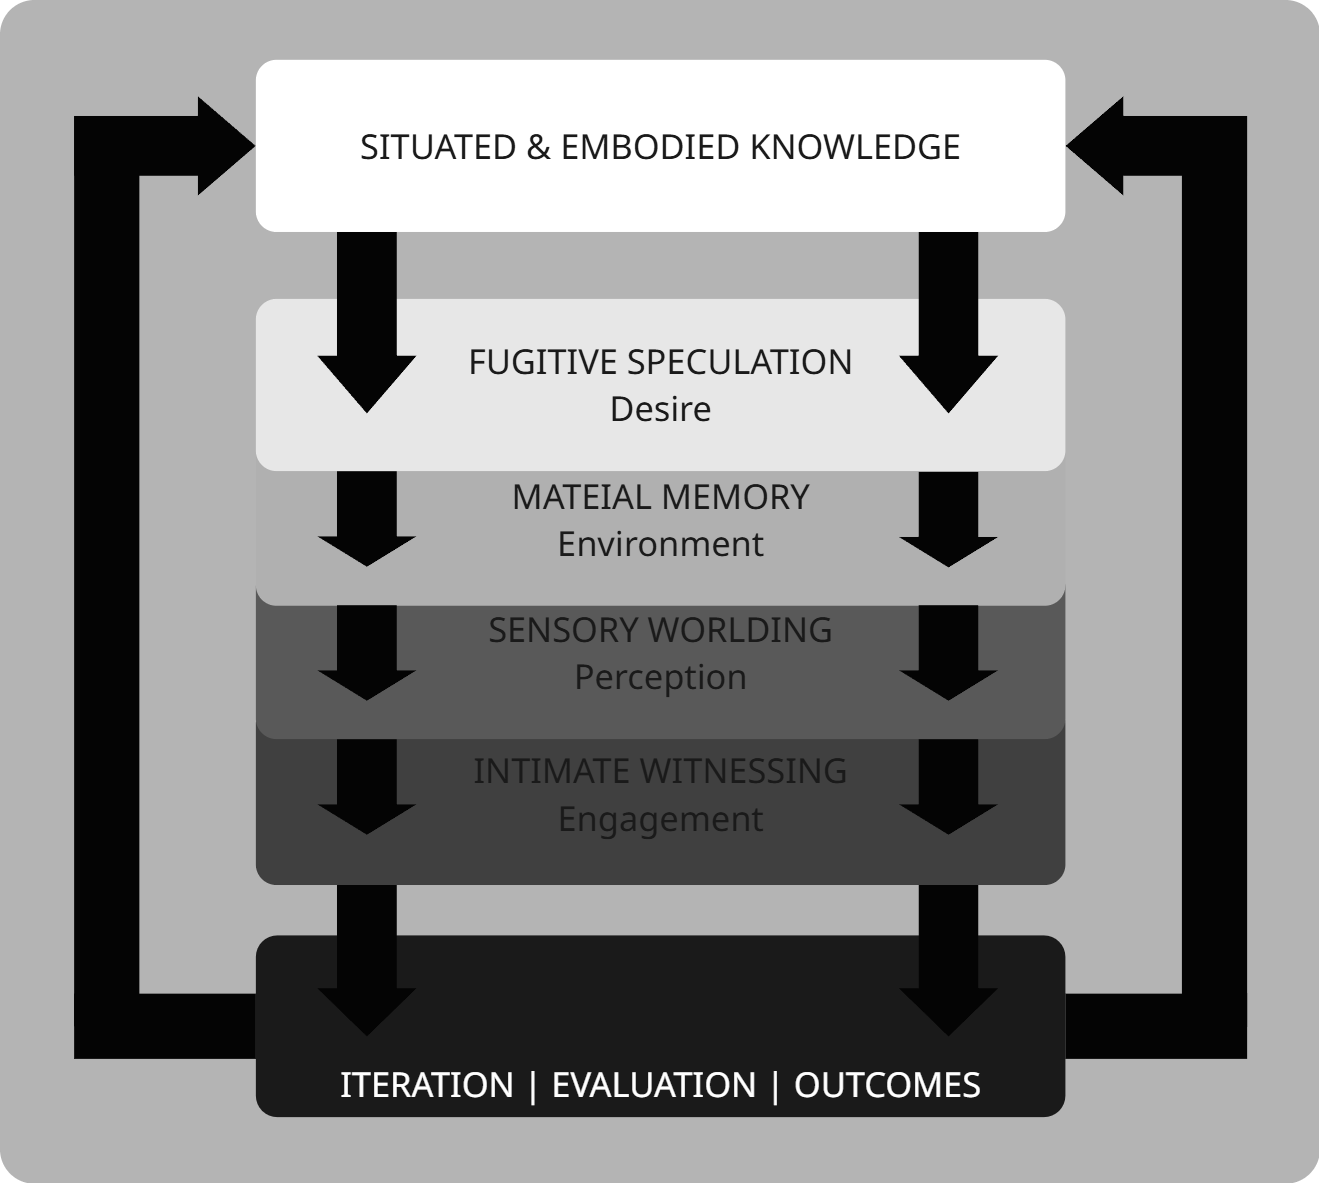
\includegraphics[width=.85\textwidth]{assets/figures/st_domains.png}
	\caption{The four main domains of cultural-technical integration within ST}
	\label{fig:main-domains}
\end{figure}

\subsubsection{Fugitive Speculation}
\noindent Fugitive Speculation acknowledges that marginalized epistemologies often operate speculatively as survival strategies, a specific desire, or necessity. Interestingly enough, \emph{modification} also, arises from a similar place. The purpose of this form of speculation is often to imagine technological futures from cultural positions systematically excluded from dominant design paradigms. This domain demands that speculative work remain accountable to specific cultural contexts rather than claiming false universality.

\subsubsection{Material Memory}
\noindent Material Memory recognizes that embodied knowledge is sedimented in habitual gestures, muscle memory, and sensory preferences developed through years of lived experience and cultural practice within the lived environment. Thus, research procedures must create space for these fragments somatic knowledge to guide technical modifications. They must not be overridden by predetermined frameworks. 

\subsubsection{Sensory Worlding}
\noindent Sensory Worlding attends to how different cultural traditions organize multisensory experience differently, requiring that tool modification emerge from culturally specific ways of listening, moving, and sensing. We must never assume perceptual norms or universality.   

\subsubsection{Intimate Witnessing}
\noindent  Intimate Witnessing establishes that knowledge validation cannot occur through distanced objectivity because to make distanced observations is to often err and make assumptions. Instead we should work through what Sengers et al. call "dialogic engagement," vulnerable, accountable sharing with users, collaborators, and a community who can recognize the authenticity and experiential resonance of the outcomes \parencites[56]{Sengers_2004}.